\documentclass{article}
\usepackage{fullpage}
\usepackage[czech]{babel}
\usepackage{amsfonts}
\usepackage{graphicx}
\usepackage{caption}

\title{\vspace{-2cm}Předminulý čas\vspace{-1.7cm}}
\date{}
\author{}

\begin{document}
\maketitle
\begin{itemize}
  \item Když mám dva děje v minulosti - když se něco stalo a ještě předtím se stalo něco jiného tak tehdy použijeme předminulý
\end{itemize}
\section{Tvoření}
\begin{itemize}
  \item Jako předpřítomný, ale pomocné sloveso \textit{haber} dáme do imperfekta a tedy příčestí minulé, stejné jako u předpřítomného
\end{itemize}
AAAAAA TABULKAAAAAAAA
\begin{figure}[h]
    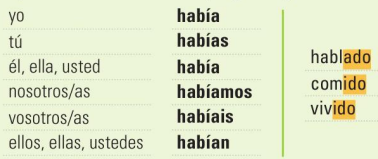
\includegraphics[width=\linewidth]{\images\predminuly_tabulka.png}
    \caption{}
\end{figure}

\section{Využití}
AAAAAAAAAAAA
\section{Příklady}
\begin{itemize}
  \item Cuando llegué al aeropuerto el avión ya había salido.
  \item Cuando llegué al banco ya había cierto.
  \item Cuando llegué a la cocina la comida había incendiado.
  \item Cuando estaba esperaba en el restaurante a Martha vi que me la había escrito.
  \item Cuando llegué a la reunión vi que la reunión ya había empezado.
  \item Cuando llegué a casa mi hija había dormido.
\end{itemize}

\section{Souslednost}
\begin{itemize}
  \item Jako v AJ
  \item Děje probíhají současně (hlavní - vedlejší), následně (hlavní -> vedlejší), nebo předčasně (hlavní <- vedlejší)
  \item V přítomnosti I. opř opř II. opř. fut. III. opř. min. (předp., jednod. i imperf.)
  \item V minulosti I. min. jednod. opř./imperf. II. min. jednod. fut./př. podmiňovací III. min. jed. min jed./imperf. (tady přímá řeč/nepřímá řeč)
  \item pozn. časy odrážky 4 ne podle časové souslednosti, ale první čas hlavní věta, druhý čas vedlejší (okolnost, dle odrážky 3))
  \item Když převádíme do minulosti z přítomnosti tak římskou číslici na římskou číslici, podobně v nepřímé řeči, tm ještě zájmena
  \item OBRAZEKOBRAZEK viz dominik
\end{itemize}
\end{document}
